%!TEX root = ../rapport.tex

\chapter{Phase de tests simple}
La phase de tests dite simple va me permettre de prendre en main les éléments de base. La situation est la suivante: 
J'utilise une tablette Nexus 7 de Asus tournant sur Android pour simuler la Set-Top Box. Celle-ci est connectée en Wifi sur le réseau local de Wingo. L'attribution des informations du réseau est fourni via DHCP. La passerelle par défaut fera donc office de routeur du client.

\begin{figure}[H]
      \centering
      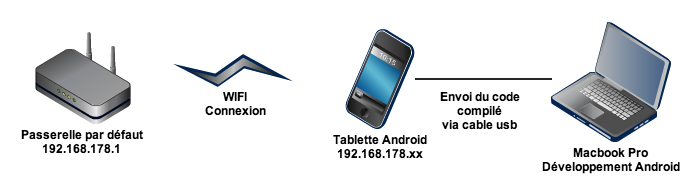
\includegraphics[width=\textwidth]{00_media/env_developpement}
      \caption{Environnement de développement simple}
      \label{gra:maqmenu}
\end{figure}

\section{Démarrage d'un service}
Qu'est-ce qu'un service sous Android? C'est un composant permettant à l'application de travailler sans interaction avec l'utilisateur. Il est donc exécuté en arrière-plan, à un moment donné. Ce moment est un événement. Dans notre cas il s'agira de démarrer le service lorsque la box aura démarrée.

\medskip

Dans un premier temps, nous devons accorder au niveau du Manifest la permission de recevoir l'événement de fin de démarrage.

\begin{lstlisting}[language=XML, caption={Permission de fin de démarrage}]
<uses-permission android:name="android.permission.RECEIVE_BOOT_COMPLETED" />
\end{lstlisting}

\medskip

Ensuite, nous devons définir un \textbf{Broadcast Receiver}, qui permet de recevoir des \textbf{Intents}, des intentions. L'intention sera "Au démarrage". Lorsque l'intention est arrivée, on lance notre service correspondant. Tout cela se passe dans le fichier AndroidManifest.xml, qui est la structure de notre application.

\begin{lstlisting}[language=XML, caption={Broadcast Receiver et Service dans AndroidManifest.xml}]
<receiver android:name="ch.wingo.stb.receiver.AutoStart" >
	<intent-filter>
		<action android:name="android.intent.action.BOOT_COMPLETED" />
	</intent-filter>
</receiver>
<service android:name="ch.wingo.stb.service.AutoStartService" android:enabled="true" />
\end{lstlisting}

La balise "receiver" permet de déclarer un BroadcastReceiver. Le nom de sa classe correspondante est "AutoStart". A l'intérieur nous avons un Intent sur l'action "BOOT\_COMPLETED". Ainsi, lorsque cette action sera filtrée, la méthode "onReceive" de la classe "AutoStart" sera exécutée.

Nous voyons aussi le service "AutoStartService". Il est juste déclaré, et ne réagit pas spécialement. C'est au rôle du receiver de lancer le service.

\begin{lstlisting}[language=Java, caption={Classe AutoStart.java}]
public class AutoStart extends BroadcastReceiver{
	private final String TAG="wingo.stb.qos.AutoStartBroadcastReceiver";
	@Override
	public void onReceive(Context context, Intent intent) {
		Intent intentToService = new Intent(context, AutoStartService.class);
		context.startService(intentToService);
		Log.i(TAG, "Service launched from AutoStart");
	}	
}
\end{lstlisting}

Comme dit précédemment, lorsque l'Intent est filtrée, la méthode "onReceive" du receiver correspondant est exécutée. C'est ici que notre Service va être lancé, via la méthode "startService". A présent, AutoStartService est lancé et c'est à partir de là que notre application commence réellement son travail!

\section{Ping}
Dans un premier temps, j'ai cherché une qualité simple à effectuer, le temps de réponse. Celui-ci peut se mesurer grâce à la commande "Ping", qui pourra aussi être utilisé pour déterminer le nombre de paquets perdus.

\medskip

Ce qui va être fait, c'est qu'au démarrage de la tablette, notre service sera lancé, puis il exécutera la commande ping sur la passerelle par défaut. Le résultat sera affiché via un Toast d'Android. Différents éléments sont nécessaires au fonctionnement du ping sur Android.

\begin{figure}[H]
    \begin{center}
        \centering 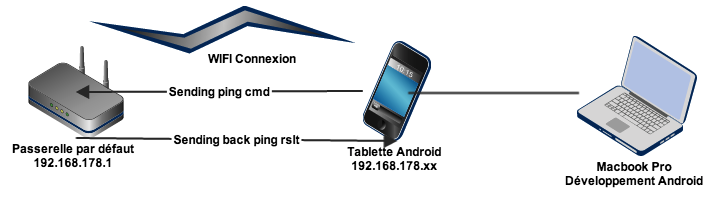
\includegraphics[width=\textwidth]{00_media/schema_ping}
        \caption{Schéma de production actuel}
    \end{center}
\end{figure}

\subsection{Runtime and Process}
La classe Runtime sur Android permet à Java d'interagir avec l'environnement sur lequel il tourne. Android est basé sur un noyau Linux, il est donc possible d'interagir avec celui-ci.
La méthode "getRuntime()" retourne l'instance unique Runtime, puis sa méthode "exec" permet d'exécuter une commande UNIX, dans un process séparé. Celui-ci est récupéré par un objet de classe "Process" et nous pouvons récupérer son flux, à savoir le résultat de la commande exécutée.

Nous sommes donc capables d'exécuter la vraie commande Ping exécutée par le Linux d'Android.

\subsection{Wifi Manager}
La classe \textbf{WifiManager} va nous permettre d'accéder à différentes informations concernant la connexion Wifi établie. Cela va de la vitesse de la connexion, à son adresse ip, ou encore toutes les informations du DHCP, comme la passerelle ou les DNS. Il est donc tout à fait possible de récupérer l'adresse IP de la passerelle pour lui lancer la commande Ping.

\subsection{Implémentation}
\subsubsection{Récupérer l'adresse IP de la passerelle par défaut}
\begin{lstlisting}[language=Java, caption={Code de récupération de la paserelle par défaut}]
//If connected to Wifi, return the gateway ip addr
	public static String getWifiDefaultGateway(){
		// getting the WifiManager from context
		WifiManager wifi = (WifiManager) STBContext.getAppContext().getSystemService(Context.WIFI_SERVICE);
		// returning the gateway converted to String, readable like an ip address
		return intToIp(wifi.getDhcpInfo().gateway);
	}
	
	// Convert int format to string ip
	// method from http://stackoverflow.com/questions/5387036/how-to-get-gateway-and-subnet-mask-details-in-android-programmatically
	public static String intToIp(int addr) {
		return ((addr & 0xFF) + "." + ((addr >>>= 8) & 0xFF) + "."
				+ ((addr >>>= 8) & 0xFF) + "." + ((addr >>>= 8) & 0xFF));
	}
\end{lstlisting}

\medskip

La méthode "wifi.getDhcpInfo().gateway" retourne un entier pour l'adresse IP. Il s'agit en fait de chaque entier de l'adresse IP, chaque fois décalé de 8 bits et converti en binaire, puis additionné. Le schéma suivant illustre la situation.
\begin{figure}[H]
      \centering
      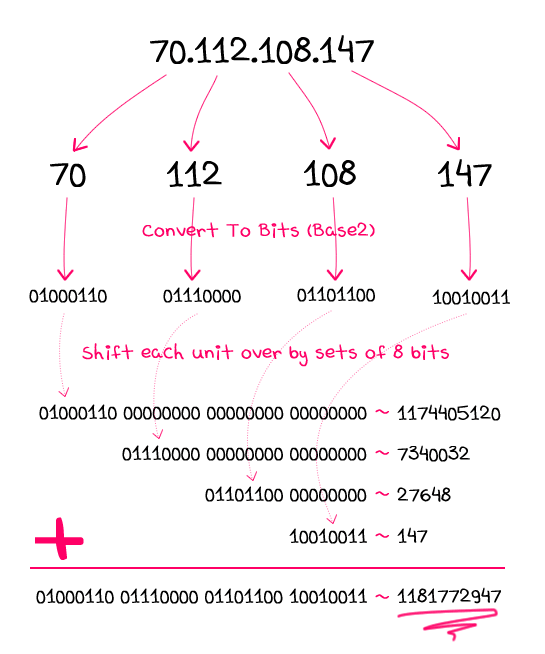
\includegraphics[height=250px]{00_media/intToIp}
      \caption{Explication sur l'adresse IP format numérique}
      \label{gra:maqmenu}
\end{figure}

La méthode "intToIp" permet de convertir un entier en String sous la forme d'une adresse IP standard.

\subsubsection{Ping}
\begin{lstlisting}[language=Java, caption={Code du ping}]
@Override
	public void onStart(Intent intent, int startid) {
		Log.d(TAG, "Service onStart");
		ping();
	}

// execute ping command
// code from http://learn-it-stuff.blogspot.ch/2012/01/ping-code-for-android-activity.html
public void ping(){
	try {
		String pingCmd = "ping -c 5 " + NetworkUtils.getWifiDefaultGateway();
		String pingResult = "";
		// getting the runtime
		Runtime r = Runtime.getRuntime();
		// executing our command ping
		Process p = r.exec(pingCmd);
		//getting the stream of the process
		BufferedReader in = new BufferedReader(new
		InputStreamReader(p.getInputStream()));
		String inputLine = "";
		String result = "";
		// building the result
		while ((inputLine = in.readLine()) != null) {
			pingResult += inputLine;
		}
		in.close();
		
		// showing the result
		Toast.makeText(this, pingResult, Toast.LENGTH_LONG).show();
	}
	catch (IOException e) {
		Toast.makeText(this,e.getLocalMessage(), Toast.LENGTH_LONG).show();
	}
}
\end{lstlisting}

Comme expliqué, nous utilisons Runtime pour exécuter un processus. Nous récupérons ensuite le flux de sortie de celui-ci afin de construire le résultat, qui sera ensuite affiché sur un Toast.
\section{Iperf}
\begin{shadequote}
Iperf est un outil pour mesurer la bande passante et la qualité d'un lien réseau. Ce dernier est délimité par deux machines sur lesquelles est installé Iperf.
\par\emph{Définition tirée de OpenManiak.com}
\end{shadequote}

Iperf va donc être utilisé pour mesurer la bande passante. Il sera lancé en tant que serveur sur notre serveur, et en tant que client sur notre terminal Android.

\medskip

Nous allons utiliser \textbf{Iperf for Android}, qui est une version recompilée et adaptée à l'architecture d'Android. Nous aurons ainsi le vrai outils Iperf, qui sera presque utilisé de la même manière que le ping.

\medskip

Iperf for Android propose son code source, une interface graphique ainsi que le code permettant de lancer la commande et lire le résultat.

\subsection{Implémentation}

Voici la méthode permettant l'exécution d'Iperf.

\begin{lstlisting}[language=Java, caption=Code d'exécution d'Iperf]

public String iperf(){
Process process = null;
		try {
			// getting the server from the ressource file
			String cmd = "-c " + getString(R.string.server_addr_ip)
					+ " -i 10";
			// split the command
			String[] commands = cmd.split(" ");
			List<String> commandList = new ArrayList<String>(
					Arrays.asList(commands));
					
			// The execution command is added first in the list for the shell
			// interface.
			commandList.add(0, getString(R.string.iperf_data_folder));

			// Creating and running the process with our iperf
			process = new ProcessBuilder().command(commandList).redirectErrorStream(true).start();
			
			// A buffered output of the stdout is being initialized so the iperf
			// output could be displayed on the screen.
			BufferedReader reader = new BufferedReader(new InputStreamReader(
					process.getInputStream()));
					
			String str1 = "";
			String iperfResult = "";

			while ((str1 = reader.readLine()) != null) {
				iperfResult += str1+"\n";
			}
			reader.close();
			process.destroy();
			Log.d(TAG, "Iperf result: \n" + iperfResult);
		} catch (IOException e) {
			Log.e(TAG, e.getMessage());
			return "";
		}
		return iperfResult;
	}
\end{lstlisting}

Ce que nous remarquons c'est que cette fois nous n'utilisons pas le Runtime car la commande ne vient pas du noyau Linux mais c'est un exécutable qui se trouve dans les sources du projet. Ainsi, au lieu de récupérer le processus via le Runtime, nous allons créer celui-ci via l'objet \textbf{ProcessBuilder}. Sa méthode "command" prend en paramètre une liste. Celle-ci est en fait la séparation de toutes les options de la commande.

\begin{table}[H]
\begin{tabularx}{\textwidth}{|m{3cm}|X|l|}
  \hline
  \bf{Position} & \bf{Valeur} \\
  \hline
  0 & /data/data/ch.wingo.stb/iperf \\
  \hline  
  1 & -c\\
  \hline  
  2 & http://addr\_server \\
  \hline  
  3 & -i \\
  \hline  
  4 & 10\\
  \hline
\end{tabularx}
\caption{Contenu de la liste de commandes pour iperf}
\label{tab:classDiagram}
\end{table}

\medskip

Ainsi, la commande effectuée est "/data/data/ch.wingo.stb/iperf -c http://addr\_server -i 10".

\medskip

A noter que le répertoire \textbf{ch.wingo.stb} correspond au nom du package et que c'est le seul endroit possible pour une application de stocker des informations qui lui sont propres. Ainsi, l'exécutable iperf pour Android est copié dans ce répertoire lors de sa première utilisation. Lors de mes premières tentatives d'exécution le répertoire était faux, ce qui empêchait la copie d'iperf.
\begin{figure}[H]
      \centering
      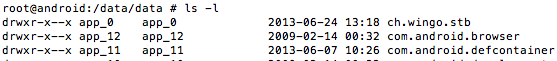
\includegraphics[width=350px]{00_media/droit_repertoire_data}
      \caption{Liste des droits dans le répertoire data d'Android}
      \label{gra:maqmenu}
\end{figure}

\medskip

On voit que seul l'utilisateur app\_0, créé pour notre application, a accès à ce répertoire. Et il est impossible d'en utiliser d'autres.

\medskip

L'option -i permet quant à elle de définir sur combien de secondes la mesure va être faite.

\section{Hello World Serveur}
La dernière partie de la phase de tests simple était de mettre en place le serveur et de communiquer de manière simple avec notre terminal Android.

\subsection{Installation de Jetty}
Jetty est téléchargeable sur son site officiel.

http://download.eclipse.org/jetty/stable-9/dist/

\medskip

Nous nous retrouvons avec une archive à dézipper qui contient le serveur.

\medskip

La structure est la suivante:
\begin{figure}[H]
    \begin{center}
        \centering 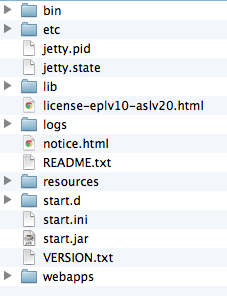
\includegraphics[width=120px]{00_media/jetty_arb}
        \caption{Jetty structure}
    \end{center}
\end{figure}

\begin{table}[H]
\begin{tabularx}{\textwidth}{|m{3cm}|X|l|}
  \hline
  \bf{Répertoire} & \bf{Description} \\
  \hline
  bin & Contient les exécutables de Jetty. On y trouve notamment \textbf{Jetty.sh} qui permet, via les options start, stop et restart de démarrer, stopper et redémarrer le serveur \\
  \hline  
  etc & Contient tous les fichiers de configuration de Jetty. Par défaut peu utile, mais pour la mise en place d'SSL c'est ici que nous irons.\\
  \hline  
  lib & Contient toutes les librairies de Jetty\\
  \hline  
  logs & Contient tous les fichiers de logs. Chaque jour un nouveau log est créé. \\
  \hline  
  resources & Contient quelques fichiers de configuration en rapport aux logs notamment. \\
  \hline
  start.d & Dossier de démarrage de Jetty. Il contient par défaut le lancement de l'application démo de Jetty, à supprimer lors de la mise en production car vulnérable! \\
  \hline
  webapps & Dossier de déploiement de Jetty. Les applications sont à déposer ici avec d'être automatiquement déployées par Jetty. \\
  \hline
\end{tabularx}
\caption{Arborescence du répertoire de Jetty}
\label{tab:classDiagram}
\end{table}

\medskip

Pour lancer Jetty, il suffit à présent de se placer depuis le terminal dans son répertoire et de lancer la commande 

\begin{lstlisting}[caption={Commande de lancement de Jetty}]
bin/jetty.sh start
\end{lstlisting}

\medskip

Si tout s'est bien passé, rendez-vous sur la page \textbf{http://localhost:8080} afin de voir la page d'accueil de Jetty.

\begin{figure}[H]
      \centering
      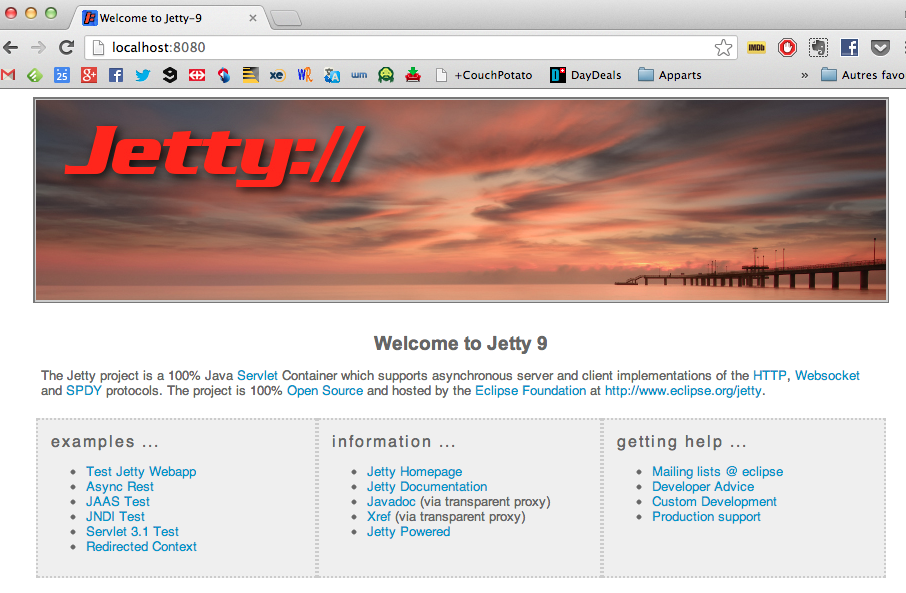
\includegraphics[width=\textwidth]{00_media/welcome_jetty}
      \caption{Page d'accueil du serveur Jetty}
      \label{gra:maqmenu}
\end{figure}

\medskip

Notre serveur tourne !

\subsection{Implémentation du serveur}
Nous allons voir ici ce qui est nécessaire au fonctionnement basique des WebSockets sur notre serveur.

Concrètement, nous avons besoins de deux choses:
\begin{enumerate}
	\item Une servlet permettant la réception des requêtes de connexion et la création d'un socket dédiée
	\item Un socket permettant de dialoguer avec notre terminal Android.
\end{enumerate}

\medskip

C'est tout ce qu'il faut. Au niveau de l'implémentation, plusieurs possibilités s'offrent à nous. Utiliser les fichiers de configuration, utiliser les annotations ou instancier chaque classe nous-mêmes.

J'ai personnellement choisi l'annotation, pour la clarté offerte. Lorsque l'on voit la classe, on sait directement à quoi elle va servir, pas besoin de vérifier dans un fichier de configuration externe, et pas besoin de créer des possibilités d'erreurs en créant le tout nous-mêmes.

\medskip

Nous allons ici faire le tutoriel proposé par Eclipse permettant de faire un \textbf{echo}. Chaque message réceptionné par le serveur sera renvoyé en retour au client.

http://www.eclipse.org/jetty/documentation/current/jetty-websocket-api-annotations.html

\subsubsection{Servlet}
Notre servlet nous sert à réceptionner les requêtes HTTP désirant établir une connexion WebSocket sur notre serveur. On devra donc lui définir une \textbf{URL}.

\medskip

La réception faite, il s'agit ici de configurer quelque peu le serveur. Nous allons ici juste lui donner un \textbf{idleTimeout}, un timeout qui coupera la connexion si aucun trafic n'a été détecté durant un certain temps. Ce temps sera de \textbf{10 minutes}. Cette valeur sera stockée dans le fichier web.xml afin d'être facilement modifiable.

\medskip

Ensuite, nous créerons un socket qui s'occupera de communiquer avec notre terminal.

\begin{lstlisting}[language=Java, caption={Servlet de réception de requêtes HTTP}]
@SuppressWarnings("serial")
@WebServlet(name="PRIS WebSockets", urlPatterns="/register")
public class RemoteSTBServlet extends WebSocketServlet {
 
    @Override
    public void configure(WebSocketServletFactory factory) {
    	// getting the idleTimeout parameter from web.xml
    	int idleTimeout = Integer.parseInt(getServletContext().getInitParameter("idleTimeout"));
    	System.out.println(new Date()+" Servlet: configured ! Timeout set to "+idleTimeout+" ms");
    	// setting the timeout
    	factory.getPolicy().setIdleTimeout(idleTimeout);
    	// creating a new Socket
        factory.register(RemoteSTBSocket.class);
    }
}
\end{lstlisting}

Pour résumer les quelques paramètres

\begin{table}[H]
\begin{tabularx}{\textwidth}{|m{3cm}|X|l|}
  \hline
  \bf{Répertoire} & \bf{Description} \\
  \hline
  @WebServlet & Annotation définissant la classe comme Servlet \\
  \hline  
  name & Nom de la Servlet\\
  \hline  
  urlPatterns & URL d'accès à la Servlet. L'URL est relative à l'adresse de l'application.\\
  \hline  
  extends WebSocketServlet & Étend à la classe WebSocketServlet qui nous donne accès à la méthode "configure". Celle-ci sera ensuite exécutée automatiquement.\\
  \hline  
  factory.register & Va créer un nouveau Socket. En donnant la classe de celui-ci, l'instantiation se fait automatiquement. \\
  \hline
\end{tabularx}
\caption{Résumé des paramètres Servlet}
\label{tab:classDiagram}
\end{table}

\subsubsection{Socket}

Les Sockets permettent de communiquer entre deux points, client et serveur, via la session qu'ils gèrent. C'est ici que l'on pourra envoyer des messages sur nos terminaux, et c'est ici que l'on réceptionnera les leurs.

\medskip

Il existe 4 événements dans un Socket:
\begin{enumerate}
	\item \textbf{On Connect} : Lorsqu'un client est connecté pour la première fois
	\item \textbf{On Close}: Lorsque la connexion est fermée
	\item \textbf{On Message}: Lorsque le serveur reçoit un message du client
	\item \textbf{On Error}: Lorsqu'une erreur survient.
\end{enumerate}

Ces événements sont interceptés par les annotations. Nous aurons par exemple \textbf{@OnWebSocketConnect} pour définir la méthode qui réceptionnera l'événement "On Connect".

\medskip

Chaque méthode prend en paramètre un objet de type Session, qui est l'objet de connexion avec le client distant. Via cet objet nous pourrons donc envoyer des messages mais aussi fermer la connexion, savoir si la session est ouverte, si elle sécurisée, quelle est l'adresse IP du client etc.

\medskip

Voici le code permettant de faire un "echo" d'un message reçu.

\begin{lstlisting}[language=Java, caption={Code du Socket pour faire un echo}]
@WebSocket(maxMessageSize = 64 * 1024)
public class EchoSocket {
 
    @OnWebSocketMessage
    public void onText(Session session, String message) {
        if (session.isOpen()) {
            System.out.printf("Echoing back message [%s]%n", message);
            session.getRemote().sendStringByFuture(message);
        }
    }
}
\end{lstlisting}

Donc ce qu'on peut lire c'est: 

"Lorsque je reçois un message, je vérifie que la session soit bien ouverte. Si c'est le cas, je renvoie le message dans le futur au client".

\medskip

\textbf{session.getRemote()} me permet de récupérer un objet "RemoteEndpoint", qui correspond à mon interlocuteur.

\textbf{sendStringByFuture} va envoyer un message, mais de manière \textbf{non bloquante}. C'est-à-dire qu'une pile de messages existe et que notre message y est ajouté, en étant envoyé sans qu'on ne sache à quel moment. En opposition il existe \textbf{sendString} qui lui est \textbf{bloquant}. Le message est directement envoyé et le code continue uniquement lorsque celui-ci a été réceptionné par le client.

\subsection{Résultat du serveur}
Après quelques recherches, j'ai trouvé un utilitaire se nommant \textbf{Dark WebSocket Terminal}
 permettant de se connecter à un serveur en utilisant les WebSockets. Il va ainsi me permettre de tester si mon serveur est bien configuré.
 
https://chrome.google.com/webstore/detail/dark-websocket-terminal/

\subsection{Implémentation du client}
Du côté du client, comme expliqué en "Analyse", nous allons utiliser \textbf{Autobahn Android}. Son utilisation se veut simple: un objet \textbf{WebSocketConnection} mConnect, contenant la méthode \textbf{connect}, et prenant en paramètre l'URL du serveur ainsi qu'une instance de la classe \textbf{WebSocketHandler} qui elle réceptionnera les différents événements, comme vu avec les Sockets.

\medskip

Les événements sont les suivants:

\begin{enumerate}
	\item onOpen : Ouverture de la connexion
	\item onTextMessage: Lors de la réception d'un message texte
	\item onClose: Lors de la fermeture de la connexion
\end{enumerate}

L'envoi de message sur le serveur se fait via la méthode \textbf{sendTextMessage} de l'objet mConnect.

\medskip

Ce que nous allons simplement faire, c'est envoyer le message "Hello World" au démarrage du terminal, qui devra être renvoyé en retour par le serveur.

\begin{lstlisting}[language=Java, caption={Envoi Hello World Android vers Serveur via WebSockets}]

   private final WebSocketConnection mConnection = 
   new WebSocketConnection();

   @Override
      public void onStart(Intent intent, int startid) {
            connectToServer();
      }
      
   public void connectToServer(){
      try {
      // connecting to the IP of my server in the local network
      String wsuri = "ws://192.168.0.10:8080/qosServer/register";
      mConnection.connect(wsuri, new WebSocketConnectionHandler() {
         @Override
         public void onOpen() {
            Log.d(TAG, "Connected to serveur");
            //sending hello world
            mConnection.sendTextMessage("Hello World !");
         }

         @Override
         public void onTextMessage(String payload) {
            Log.d(TAG, "We have got a message:\n");
            Log.d(TAG, payload);
         }

         @Override
         public void onClose(int code, String reason) {
            Log.d(TAG, "Closing the connection. Reason: "+reason);
         }
      });
   } catch (WebSocketException e) {

      Log.e(TAG, e.toString());
   }
}
\end{lstlisting}

\medskip

L'url a été construite comme expliquée: 

l'adresse IP du serveur, qui sera remplacée dans le futur par un nom de domaine + 

le nom du fichier déployée sans l'extension (qosServer.war) + 

l'url de la servlet (/register).